\documentclass[12pt]{iopart}

% packages
\usepackage{graphicx}
\usepackage{IEEEtrantools}
\usepackage{amsmath}

% Custom macros
\gdef\mcm{r@{.}l@{ ± }r@{.}l} % Multi Column Measurement; Used for decimal aligning & ± aligning
\gdef\mch#1{\multicolumn{4}{l}{#1}} % Multi Column Header; Used for decimal aligning & ± aligning
\gdef\mcmnd{r@{ ± }l} % Multi Column Measurement No Decimal; Used for ± aligning when the values don't need a decimal point
\gdef\mchnd#1{\multicolumn{2}{l}{#1}} % Multi Column Header No Decimal; Used for  ± aligning when the values don't need a decimal point
\gdef\sci#1#2{#1 \times 10^{#2}}
\gdef\units#1{~\mathrm{#1}}
\graphicspath{{./images/}}

%%%%%%%%%%%%%%%%%%%% Document Starts %%%%%%%%%%%%%%%%%%%%
\begin{document}

%%%%%%%%%%%%%%%%%%%% Title Page %%%%%%%%%%%%%%%%%%%%
\title{DTMF Signaling}
\author{Ali Mortada, Xavier Valencia, James Phommachanh}
\vspace{10pt}
\begin{indented}
  \item[]Mt.~San Antonio College, ENGR 285, CRN 43464
  \item[]June 14, 2024
\end{indented}
\newpage

%%%%%%%%%%%%%%%%%%%% Objective 1 %%%%%%%%%%%%%%%%%%%%
\section{Objective 1: Encoding Program}

%What to talk about:
%\begin{itemize}
     %What \verb|createPureToneData()| does
     %What \verb|toneList| is
    %What the for loop does
%\end{itemize}

The short and sweet explanation as to what the encoding program does is that it makes a \verb|.wav| file that contains a series of tones that are made from a list along with a series of pauses so that the original list of numbers fed into the program cannot be read without the proper decoding program.

From the top of the code, we import a few libraries to perform some math functions, then convert those outputs into \verb|.wav| files. 
We make a file name for the \verb|.wav| output, then a list of numbers that are between 0-9 to input into the program. 
The \verb|sampleRate| variable is the step size of the wave file, so a higher sample rate would allow for a more accurate replication of that particular frequency. 
There is a limit to the frequencies a human can hear, so we will not change this value. 
The variable \verb|soundLevel| represents the amplitude of the frequencies produced, so as the name of the variable indicates, a higher value will result in a higher sound level, with the contra-positive being true as well. 
The variable \verb|pauseLength| is there to help encode the frequencies so that you cannot properly playback the \verb|.wav| file.

We then create a function that will take in a frequency and create an array that loops for as long as the iterating variable is less than the sample rate value with the iterator incrementing at the end of each loop.
The array is filled with a series of points that are representative of a sine wave of the input frequency. 
We do this for a series of frequencies and store them in variables, then the different frequencies are summed into a new list so that they correspond to the table given in the order of 0-9. 

\begin{figure}[h!tbp]
  \begin{center}
 \item[]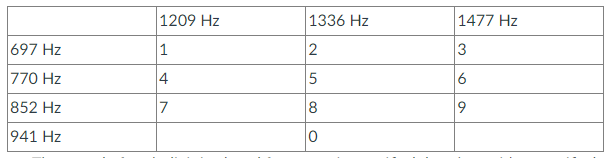
\includegraphics[width=0.6\textwidth]{images/Capture.PNG}
  \caption{\label{fig: Keypad Tones} 
  Keypad tones provided.
  }
  \end{center}
\end{figure}

This list is essentially creating new tones by using constructive wave interference and associating a number to this new tone. 
This will be called \verb|toneList| as provided. 
Now that we have a way to create a unique tone for each input and represent it in a list, we can now reference our \verb|toneList| with the inputs of our \verb|numberList|. 
We will make a new array called \verb|soundData| that adds the tone list data along with pauses between each tone. 
This will be done in a for loop for the range of the \verb|numberList|. This loops for however long the number list is, but it is noteworthy that we should increase the value of \verb|soundLength| if we increase the length of the \verb|numberList|.

Once that final for loop is done, we have all of our data to copy to the \verb|.wav| file, the IDE opens the \verb|.wav| file created prior and sets some parameters. 
These parameters include \verb|nchannels|, which is the number of audio channels. 
I don’t know how I feel about Dolby Atomos keypad tones. 
The variable \verb|sampwidth| is the number of bytes used when writing data to the \verb|.wav| file, we have 2 bytes so it would be 16 bits. 
The variable \verb|framerate| is \verb|sampleRate| but converted to an integer. The variable \verb|nframes| represents the amount of steps that the \verb|.wav| file will have, or how long it will be. The line \verb|comptype = “NONE”| tells the program not to compress the output file, and \verb|compname| is a description of the compression type. 
We set the parameters using a wave library function, then we use a for loop to write all of the data we have using a different wave library function.
Finally, it closes the file and prints a message to the terminal indicating that the program has successfully written to the output file.

% figures look like this and go into the images folder
%\begin{figure}[h!tbp]
%  \begin{center}
% \item[]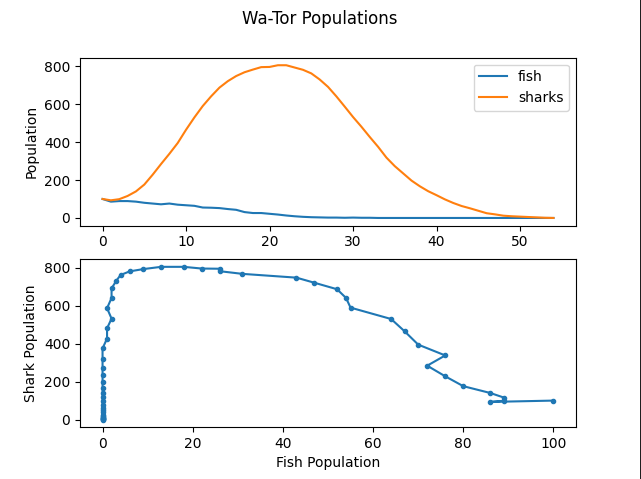
\includegraphics[width=0.6\textwidth]{figure1.png}
%  \caption{\label{fig:figure1}
%  Horizontal motion vs. time. 
%  It is clear that the horizontal motion increases as its step is increased by 3.
%  }
%  \end{center}
%\end{figure}


%%%%%%%%%%%%%%%%%%%% Objective 2 %%%%%%%%%%%%%%%%%%%%
\section{Objective 2: Slicing Data}

%%What to talk about:
%\begin{itemize}
 %   \item %Function has to divide the data into equally sized parts which depends on the number of inputs
 %   \item %Iterates through the save data with a step size of the slice size
  %  \begin{itemize}
   %     \item %%Uses another nested for loop that only adds signals that are not pauses (signal is not equal to 0)
   %     \item %%If a signal is found, it is added to the data list that the function returns%%
    %\end{itemize}
%\end{itemize}

The \verb|slice_data()| function first divides the input data into equally sized parts, which depends on the number of inputs -- this is stored in a variable called \verb|slice_size|.
Note that if the number of inputs changes, we must change the code so that it divides the input number into the correct number of equal parts.
Figure \ref{fig:slice_graph} shows how the data is divided into different slices.

\begin{figure}[h!tbp]
  \begin{center}
 \item[]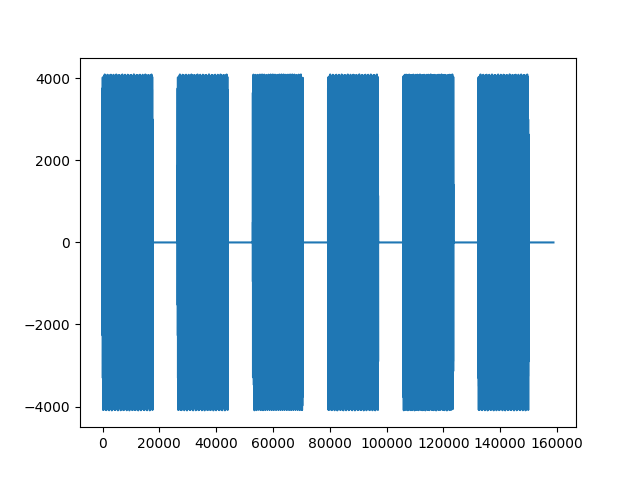
\includegraphics[width=0.6\textwidth]{images/slice_graph.png}
  \caption{\label{fig:slice_graph}
  Slice graph with input [1, 1, 2, 1, 0, 1].
  The data is divided into six equal parts, regardless of what the input values actually are.
  }
  \end{center}
\end{figure}

The function then contains a for-each loop that iterates through the length of \verb|save_data| with a step size of \verb|slice_size|.
This loop contains another nested loop that checks each data point within the slice.
If the signal is not a pause, it is added to the data list that is returned by the function, but if it is, it is skipped over. 

\begin{figure}[h!tbp]
  \begin{center}
 \item[]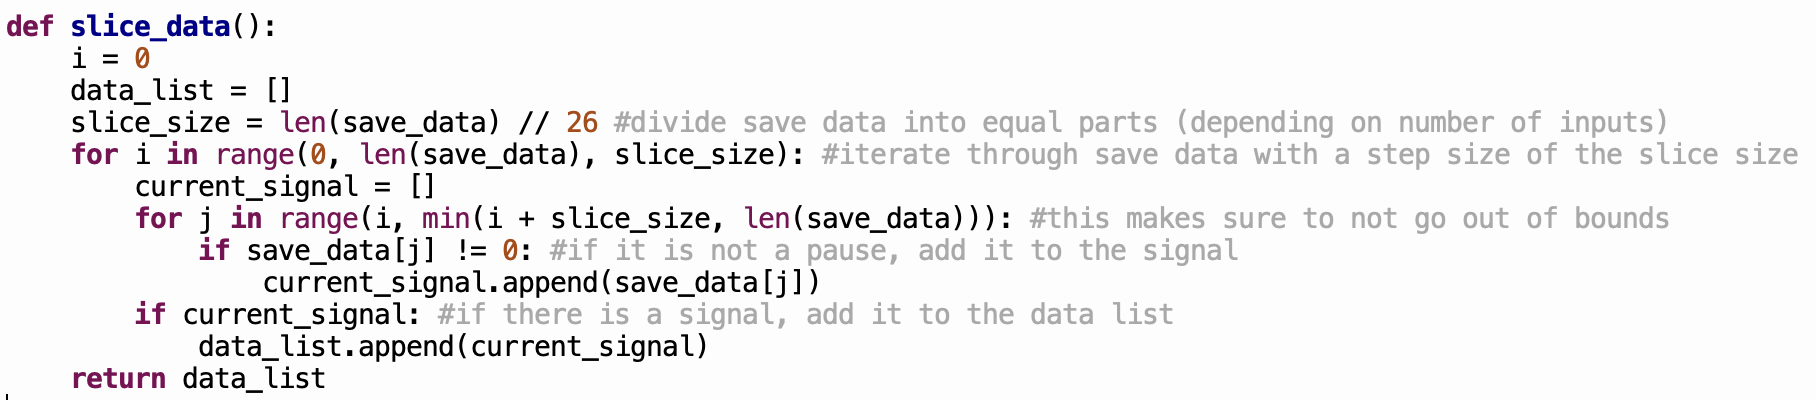
\includegraphics[width=0.9\textwidth]{images/slice_data().png}
  \caption{\label{fig:slice_data()}
  Code snippet for the slice\_data() function.
  }
  \end{center}
\end{figure}

%%%%%%%%%%%%%%%%%%%% Objective 3 %%%%%%%%%%%%%%%%%%%%
\section{Objective 3: Calculating Approximate Fourier Coefficients}

Since decoding the DTMF signals requires Fourier analysis, the Fourier coefficients can be approximated using the different decoded frequencies. 
Recall the Fourier coefficients for the sine and cosine basis:

\begin{equation}
    a_n = \frac{2}{T}\int_0^T f(t)cos(\frac{2\pi n}{T}t)\;\mathrm{d}t
\end{equation}

\begin{equation}
    b_n = \frac{2}{T}\int_0^T f(t)sin(\frac{2\pi n}{T}t)\;\mathrm{d}t
\end{equation}

The coefficients in the program correlate to each of these Fourier bases. 
Thus, an approximation of the coefficients can be calculated by taking the summation of each frequency from the sliced data for the decoded sound signal. 
The period for each Fourier Basis ($T$), is the length of the decoded and sliced frequencies. 
Then for each data point ($n$), the frequencies ($t$) within the trigonometric part of the basis are divided by the frame rate -- which in this case is the period ($T$). 
In the program, this simplifies to: 

\begin{equation}
    a_n = \frac{2}{T}\sum_{0}^{T} \mathrm{frequency} * cos(\frac{2\pi * \mathrm{data point} }{\mathrm{framerate}} * \mathrm{frequency})
\end{equation}

\begin{equation}
    b_n = \frac{2}{T}\sum_{0}^{T} \mathrm{frequency} * sin(\frac{2\pi * \mathrm{data point}}{\mathrm{framerate}} * \mathrm{frequency})
\end{equation}

This results in the approximation of the Fourier coefficients for the DTMF signaling for each of the Fourier bases. The function returns the Euclidean norm of the Fourier basis in a plane representing each of the bases.

\begin{figure}[h!tbp]
  \begin{center}
 \item[]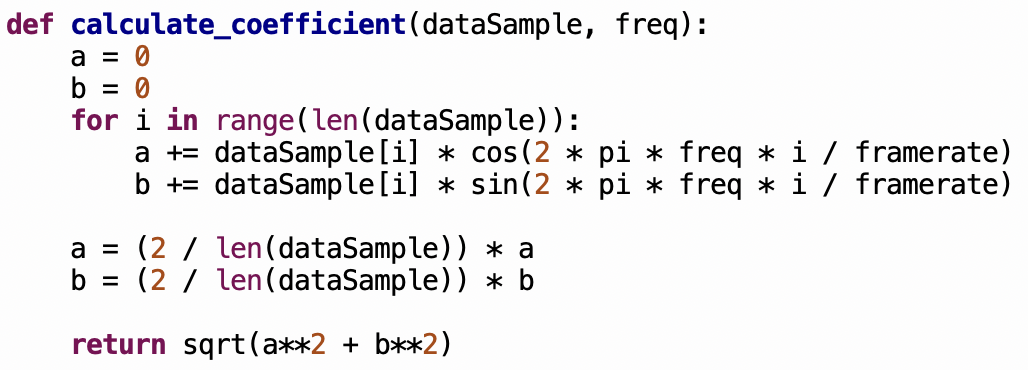
\includegraphics[width=0.8\textwidth]{images/calculate_coefficient().png}
  \caption{\label{fig:calculate_coefficient()}
  Snippet of code for the calculate\_coefficient() function.
  }
  \end{center}
\end{figure}

%%%%%%%%%%%%%%%%%%%% Objective 4 %%%%%%%%%%%%%%%%%%%%
\section{Objective 4: Outputting Decoded Digits}

To output the decoded digits, a list of the Fourier coefficients of the decoded signal list can be iterated for each of the respective high and low frequencies of the program. 
Now for each signal from the data list, there is a list of low and high Fourier coefficients. 
The max of each of the coefficients represents the true occurrence of the high and low frequencies in the data signal. 
Thus, we can store the instances of these max coefficients for each signal to decipher the decoded digits. 
Once we have a list of where these instances occur, we find an instance in this list that correlates to the decoded digit originally in the decoded list of numbers. 
To check if an instance exists to the decoded list, we only stored digits that did not return -1 when put into the \verb|decode_freqs()| function. 

\begin{figure}[h!tbp]
  \begin{center}
 \item[]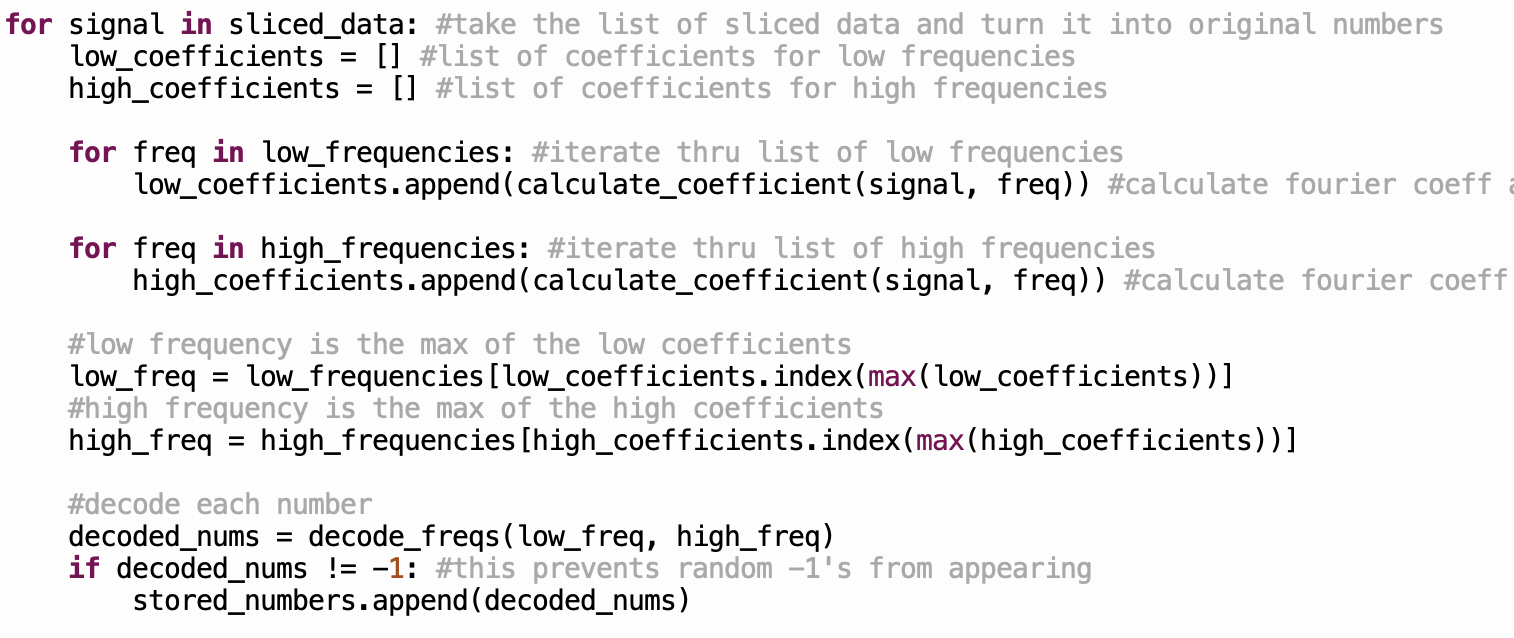
\includegraphics[width=0.9\textwidth]{images/main_for_loop.png}
  \caption{\label{fig:main_for_loop}
  The program's main for loop.
  }
  \end{center}
\end{figure}

%%%%%%%%%%%%%%%%%%%% Extension %%%%%%%%%%%%%%%%%%%%
\section{Extension: Handling Alphabetical Messages}

For the extension, we decided to implement handling alphanumeric messages (apparently we don't know how to read instructions properly).
To do this, we had to extend the list of low and high frequencies, since the original four low frequencies and three high frequencies cannot make thirty-six unique combinations.
Thus, we added two new frequencies to the low frequencies list, $1037 \units{Hz}$ and $1144 \units{Hz}$, and three new frequencies to the high frequencies list, $1633 \units{Hz}$, $1776 \units{Hz}$, and $1919 \units{Hz}$.
These frequencies were chosen arbitrarily by our good friend Chad, and Figure \ref{fig:extended_freq_table} shows the mapping of each alphanumeric symbol to its pair of low and high frequencies. 
In the \verb|DTMFwrite| program, the arrays for each frequency were replaced by a frequency map matching each symbol to its pair of frequencies, and this map was used to populate \verb|toneList|.

\begin{figure}[h!tbp]
  \begin{center}
 \item[]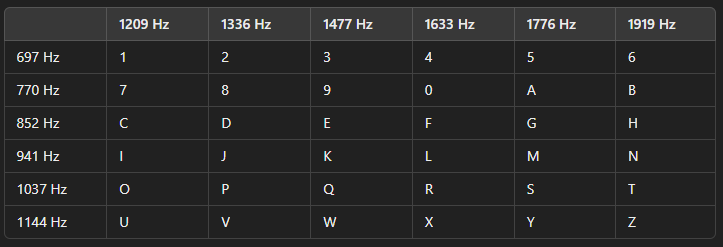
\includegraphics[width=0.8\textwidth]{extended_freq_table.png}
  \caption{\label{fig:extended_freq_table}
  Extended frequency table matching each alphanumeric symbol to a pair of low and high frequencies.
  }
  \end{center}
\end{figure}

The \verb|slice_data()| function was also slightly modified to handle more symbols.
The variable \verb|slice_size| was redefined to be smaller to ensure a more accurate tone was recorded.
New variables \verb|overlap| and \verb|sound_cutoff| were also defined to make sure the full tone was recorded and to filter out signals with no sound, respectively.
The for loop now checked to see if the current signal was above the cutoff threshold before adding it to the data list -- otherwise, it would skip over the overlap.

The code was now theoretically ready to handle alphanumeric messages.
However, when it was tested, we found that the program would output multiple copies of the same symbol for each symbol in the message, as shown in Figure \ref{fig:extension_output_bad}.
To fix this, code was added to check if the current character is equal to the previously stored character -- if it is not, then it is added to the list of stored characters.
This seemed to fix the issue, but it added the limitation of being unable to read messages that have two or more of the same symbol consecutively, only outputting one copy of the letter.
A sample output after the fix can be seen in Figure \ref{fig:extension_output}.

\begin{figure}[h!tbp]
  \begin{center}
 \item[]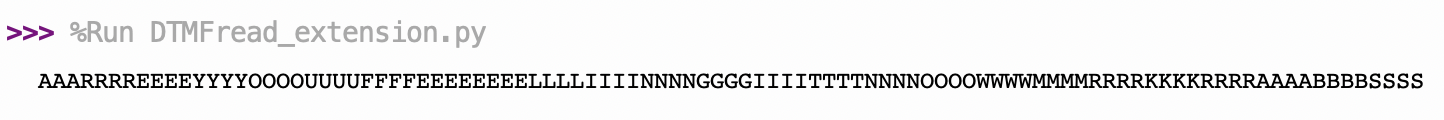
\includegraphics[width=1\textwidth]{extension_output_bad.png}
  \caption{\label{fig:extension_output_bad}
  Initial output with test message "AREYOUFEELINGITNOWMRKRABS". 
  Notice how each letter has 3-4 multiples in the output.
  }
  \end{center}
\end{figure}

\begin{figure}[h!tbp]
  \begin{center}
 \item[]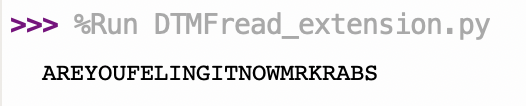
\includegraphics[width=0.6\textwidth]{extension_output.png}
  \caption{\label{fig:extension_output}
  Initial output with test message "AREYOUFEELINGITNOWMRKRABS" after fixing repeated symbol issue. Notice how the double E in "FEELING" only has one E outputted.
  }
  \end{center}
\end{figure}

It is worthy to note that after implementing this extension, it takes noticeably longer for both the \verb|DTMFread| and \verb|DTMFwrite| programs to execute.
This is likely because it has to map each symbol to its frequency pair instead of just reading from an array for each frequency.
Both programs also contain multiple nested loops, so it is not unreasonable to assume that the time complexity of each program increases quadratically with an increasing number of symbols.


\end{document}
%%%%%%%%%%%%%%%%%%%% Document Ends %%%%%%%%%%%%%%%%%%%%